\section{Temporal patterns and indexing} \label{tpatterns}
In previous sections of this chapter we have shown the PAA and SAX algorithms for conversion of real valued time series into the symbolic representation along with symbolic temporal data models, concepts and operators. All these was a necessary background in order to continue with review of approaches for unsupervised knowledge mining from a symbolic temporal data. In this section we will review sequential pattern mining algorithms from time points and time-intervals data. We will base the review on the univariate data extending it to the multivariate.


Before discussing algorithms we need to provide a formal definition of \textit{pattern}. The essential property which defines a pattern is called \textit{support}. The support, roughly speaking, is the frequency of occurrence of the certain pattern in the observed data. It is generally assumed that each of the possible patterns have a certain probability to be seen in the dataset just by a chance, this probability is called \textit{expected} probability and defines the \textit{expected support} for the pattern. When the actual observed support (or frequency) of a pattern significantly differs from the expected one, it is called \textit{significant support} and indicates that pattern might have some meaningful knowledge artifact attached to it. Although, support different from the expected one does not guarantee usefulness or interestingness, it is used for a powerful pruning of a search space since most possible patterns will not have a sufficient support. Note, that there is other property \cite{citeulike:2804633} discussed in the literature which essentially similar to support: \textit{confidence}. Usually confidence correlates with support, i.e. greater support correspond to the higher confidence.

There are two well-established categories of patterns with significant support. The first category of patterns, frequently occurring ones (with support higher than expected), is very important in many data mining areas such as medicine, motion-capture, robotics, video surveillance, meteorology and others. Patterns from this category usually named as \textit{repeated}, \textit{approximately repeated} or \textit{motifs}. The second category of patterns, contains patterns with the support lower than expected, this type of patterns named as \textit{surprise} or \textit{novelty} patterns. Novelty patterns also have a great value for many applications: for example it is important to detect unusual semi-repeated pattern in the ECG data diagnosing heartbeat abnormalities, or detecting unusual activity patterns in video surveillance recognizing a suspicious activity.

Note, that the temporal motif finding problem from symbolic data is very similar to one of the central problems in the field of Computation Biology \cite{citeulike:465665}. Many algorithms are very similar, but from other hands, in Biology, motifs are usually \textit{informative} and bear some information about evolutionary artifacts, which is not true in the field of time-series analysis \cite{citeulike:3978085}.

\subsection{Time points patterns}
According to M\"orchen, the most commonly searched pattern within univariate symbolic time series is order. This search for particular order of symbols within subsequence is called \textit{sequential pattern mining} \cite{citeulike:775528} and not necessarily requires symbols to be consecutive, usually gaps and substitution allowed.

\begin{figure}[tbp]
   \centering
   \includegraphics[height=55mm]{time-points.eps}
   \caption{The time-points patterns as explained in \cite{citeulike:1748833}}
   \label{fig:timepoints}
\end{figure}

The classical suffix tree algorithm \cite{citeulike:707616} with some modifications is a standard approach for pattern discovery from the string time-series according to Palopoli et al \cite{citeulike:5003338}, in this paper authors discussing algorithms of automatic discovery of frequent structured patterns (\textit{motifs}) in ``exact'' or ``approximate'' forms. There are two approaches usually used for the suffix tree building used: \textit{generative}, when algorithms generates all possible patterns and tests their appearance frequency \cite{citeulike:5012661} and \textit{scanning}, when the sliding window used to scan over the sequences available and construct the tree on the fly \cite{citeulike:5012661}. 

The certain limitation of the suffix-tree based algorithms is that the maximum length of a pattern needs to be specified upon tree construction since all sub-sequences of this length are generated or extracted from the time series with a sliding window. In \cite{citeulike:5003404} Jiang \& Hamilton compare traversal strategies for suffix trees: breadth-first, depth-first and the heuristic depth-first algorithms implementations for temporal data mining.

Another approach, specifically designed for the \textit{surprise pattern} finding problem, proposed by Keogh et al in \cite{citeulike:3025877}. Authors discuss methods of finding a surprise patterns from the temporal data and propose their ``TARZAN'' algorithm which is based upon suffix tree and Markov model and reporting surprising patterns occurring with a frequency substantially different from that one expected by a chance.

\subsection{Time interval patterns}
As we seen before, the duration concept is implicit in the time interval definition. Nevertheless, while defining a time-interval pattern we do not actually taking in account the length of interval abstracting interval relations to the ``border'' or ``mean points'' relations.

The \textit{containment patterns} discussed by Villafane et al in \cite{citeulike:2804633}. This type of temporal patterns found application in many areas, for example software system log mining: where it is important to see what events were happening within the resource overload time interval, or medicine: what was happening with the heartbeat within the period when patient's fever was high. Authors propose a method based on the \textit{containment graphs} which allows counting of the containment frequency based on the lattice. Authors designed a naive algorithm of the graph traversal performed incrementally by the path-size and have shown satisfiable results considering their limitations in the computational power. One of the algorithm limitations found is that it yields different patterns describing same temporal events. The example of containment patterns is shown at Figure \ref{fig:timeintervals} panel \textit{a}, this figure is borrowed from \cite{citeulike:1748833}.

\begin{figure}[tbp]
   \centering
   \includegraphics[height=75mm]{time-intervals.eps}
   \caption{The time-interval patterns from \cite{citeulike:1748833}}
   \label{fig:timeintervals}
\end{figure}

Allen's relations used in many of approaches to the mining of time-interval patterns. In \cite{citeulike:5159362} Kam \& Fu considered interval-based events where duration is expressed in the terms of end-points relations and designed a category of \textit{A1} temporal patterns based on Allen's relations but restricting the search space only to the right concatenations of intervals to existing patterns and limiting the depth of the patterns. Depending on the time-interval consideration order, this approach yields different patterns describing same events, for example on the Figure \ref{fig:timeintervals} panel \textit{b}: left pattern is \textit{(((A starts B) overlaps C) overlaps D)} whether right one is \textit{(((A before C) started by B) overlaps D)}.

\textit{Fluents}, another type of time-interval patterns based on the Allen's algebra, were introduced by Cohen in \cite{citeulike:5153756} addressing the problem of unsupervised learning of structures in time series. The formal definition given by authors stating that ``Fluents are logical descriptions of situations that persist, and composite fluents are statistically significant temporal relationships between fluents.'' Sliding window and Apriori algorithms used in this work. The \textit{Fluent learning algorithm} designed by authors was used in the analysis of the robot motion data collected by sensors and helped in the discovery of temporal patterns indicating persistent robot behavior along with problems with robot's sonar system. This algorithm expresses the same problem as A1 - it reports variations of discovered patterns as independent. Authors had to remove ``the set are variants'' manually before presenting results.

H\"{o}ppner in \cite{citeulike:5159615} demonstrates approach to association rules mining through the use of the \textit{state sequences} based on the pairwise relations of all temporal intervals according to Allen. The sliding window is used to generate sub-sequences and the duration of the pattern over the sliding window used to quantify the pattern support value. This information used in the turn in Apriori algorithm for mining rules. The experimental validation of the algorithm on the weather dataset shown ability of the approach to yield meaningful patterns.

The UTG relations were used in some work for the temporal interval patterns mining (Figure \ref{fig:timeintervals} panel \textit{d}) but according to M\"orchen \cite{citeulike:1748833} were ``criticized for the strict conditions relating interval boundaries''. Lacking ability to express the concept of coincidence, UTG patterns also place additional restriction on the interval, requiring start and end of intervals to be almost simultaneous. This makes the UTG-based methods somewhat limited, however Guimar\~{a}es in \cite{citeulike:5159924} shows, that results of targeted application of UTG-based linguistic knowledge representation to sleep-related breathing disorder can provide not only with valuable input for diagnosis, but lead to a discovery of previously unknown recurrent behaviors among patients.

As opposite to UTG, TSKR patterns provide support to a partial order and allow inclusion of the sub-intervals into the pattern which makes them more expressive than UTG and Allen's relations. \textit{TSKR Chord} patterns shown at the Figure \ref{fig:timeintervals} panel \textit{e} are mined with CHARM \cite{citeulike:769773} algorithm extended with support function counting a duration of the pattern occurrence \cite{citeulike:1748833}. \textit{TSKR Phrase} patterns, in turn, is built upon the partial order of the several Chords (\ref{fig:timeintervals} panel \textit{f}) and provides even more sensitivity and selectivity for temporal patterns mining.
